\documentclass{article}
\usepackage{graphicx} % Required for inserting images
\usepackage{tikz}
\usepackage{float}
\usetikzlibrary{shapes.geometric, arrows}

\tikzstyle{process} = [rectangle, minimum width=3cm, minimum height=1cm, text centered, draw=black]
\tikzstyle{arrow} = [thick,->,>=stealth]

\title{COP290 CLAB Report}
\author{Aditya Yadav \\ Degala Aman \\ Deepak Sagar}
\date{1 March 2025}

\begin{document}

\maketitle
\textbf{idhar vo edge cases ka add krdena}

\section{Introduction}
In this project we are making a spreadsheet which can perform basic arithmetic tasks, scrolling , sleep etc. Broadly there are two parts in this project, parsing the input and then calculating and recalculating the values of the cells. We made use of graphs and avl tree and other data structures to do the recalculations efficiently.


\section{Flow}
\begin{figure}
    \centering
    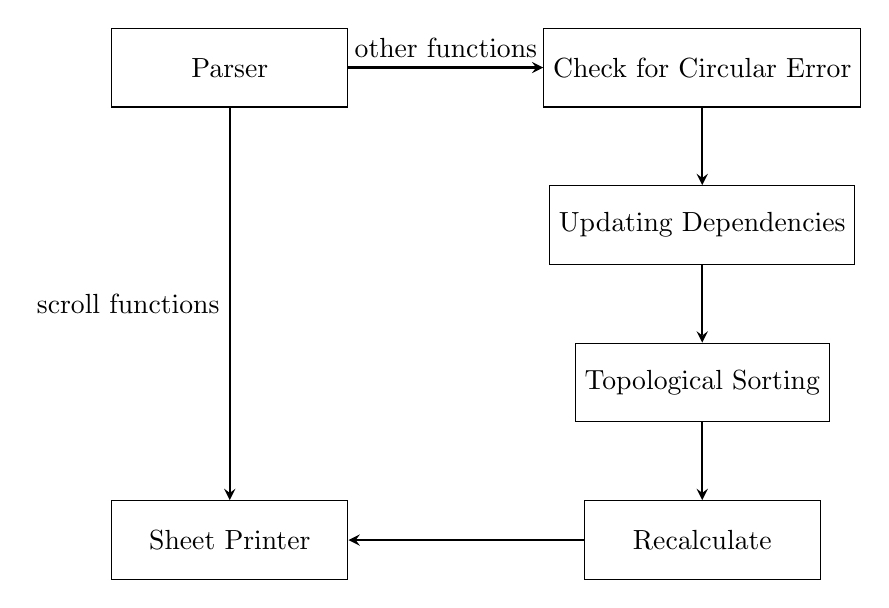
\begin{tikzpicture}[node distance=2cm]

        \node (parser) [process] {Parser};
        \node (checkError) [process, right of=parser, xshift=4cm] {Check for Circular Error};
        \node (updateDep) [process, below of=checkError] {Updating Dependencies};
        \node (topSort) [process, below of=updateDep] {Topological Sorting};
        \node (recalculate) [process, below of=topSort] {Recalculate};
        \node (printer) [process , left of=recalculate,xshift = -4cm] {Sheet Printer};

        \draw [arrow] (parser) -- (checkError) node[midway,above] {other functions};
        \draw [arrow] (checkError) -- (updateDep);
        \draw [arrow] (updateDep) -- (topSort);
        \draw [arrow] (topSort) -- (recalculate);
        \draw [arrow] (recalculate) -- (printer);
        \draw [arrow] (parser) -- (printer) node[midway,left]{scroll functions};

    \end{tikzpicture}
    \caption{Flow}
    \label{fig:1}
\end{figure}
\subsection{Parser}
Here we identify the command,take the required info from the command like the cell number and then compute the value accordingly.
We then move on to checking whether there is circular error while adding the new constraint and then updating the values and the dependencies of the cells.

\subsection{Checking for Circular Error}
We then find all the nodes that are affected by the change in value in the current node. We do this by first adding the cells that depend on the value of the current cell, then we recursively keep adding the cells that depend on this cells.We add all these cells to an AVL Tree, as all Insert and Find operations take place in O(logn) time in AVL Tree.
If in the new constraint, the current cell is dependent on value of some cell which is part of the AVL tree we created, we have a circular error and we reject the input command. 

\subsection{Updating the dependencies}
We then remove the current from the linked lists of the cells the current cell used to depend upon(if any) and add the the current cell to the linked lists of the cells which it depends upon.

\subsection{Topological Sorting}
We store an \texttt{indegree} in the node of the AVL tree which indicates the number of cells a cell's value depends on. We then use \textbf{Khan's Algorithm}
for topological sorting so that we can efficiently recalculate the value of all the cells which directly or indirectly depend on the cell to which we are adding the constraint.If we do recalculations according to the order given by this sorting, we'll be recalculating at each node only once and hence it will be efficient.

\subsection{Printing the Spreadsheet}
We then print all the cells if the output is not disabled while also printing \texttt{ERR} in place of cells which have some error.

\section{Memory}
\subsubsection{Cell Struct}
    For each cell, we have to store :-
    \begin{itemize}
        \item integer value stored in it
        \item constraint assosciated with that cell
        \item cells which depend on this cell , this is because we need to recalulate those other cells if the value in this cell changes
    \end{itemize}
    The obvious way to store these is a struct.
    The struct is as follows :
    \begin{verbatim}
        typedef struct cell{
            int value;
            bool isError;
            char op_code;
            cell_info cell1;
            cell_info cell2;
            dependency_node *dependencies;
        } Cell;
    \end{verbatim}
    The \texttt{op\_code} is a character which indicates the constraint assosciated with that cell. These are the op\_code characters and the related constraints :-
    \\\\
    \begin{tabular}{|c|c|}
        \hline
        op\_code & Constraint Type \\ 
        \hline
        =  & cell \\ 
        +  & cell + cell \\ 
        -  & cell - cell \\ 
        {*}  & cell {*} cell \\ 
        /  & cell / cell \\ 
        S  & SUM \\ 
        m  & MIN \\ 
        M  & MAX \\ 
        A  & AVG \\ 
        D  & STDEV \\ 
        Z  & sleep(cell) \\ 
        X  & const op const, const, sleep(const) \\ 
        p  & const + cell or cell + const \\ 
        s  & const - cell or cell - const \\ 
        u  & const * cell or cell * const \\ 
        d  & const / cell or cell / const \\ 
        \hline
    \end{tabular}
    \\\\
    The \texttt{cell\_info} is a struct which stores the row and column of the cells which appears in the constraints.
    \\
    \texttt{dependices} is basically a linked list storing the \texttt{cell\_info} structs of the cells which depends on the value of the current cell.  We store \texttt{(column of cell)*1000 + (row of cell)} as the value in each node in dependency list
    \\
\begin{figure}[H]
    \centering
    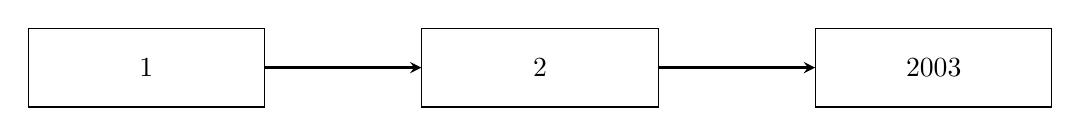
\begin{tikzpicture}[node distance=2cm]

        \node (1) [process] {1};
        \node (2) [process, right of=1, xshift=3cm] {2};
        \node (3) [process, right of =2,xshift=3cm] {2003};
 

        \draw [arrow] (1) -- (2);
        \draw[arrow] (2) -- (3);


    \end{tikzpicture}
    \caption{dependency linked list}
    \label{fig:simple-diagram}
\end{figure}

    \textbf{Memory used by cell struct}:
    \begin{itemize}
        \item value :  4 bytes
        \item isError : 1 byte
        \item op\_code : 1 byte
        \item cell1 : 4 bytes
        \item cell2 : 4 bytes
        \item dependencies : 8 bytes
    \\\\\textbf{Total} : 22 bytes
    \end{itemize}
    The \texttt{dependency\_node{*} dependencies} points to linked list which might keep increasing.

    \subsubsection{The Spreadsheet}
    The number of rows in the spreadsheet can range from 1 to 999 and the columns from A to ZZZ, Therefore the total number of cells in the spreadsheet can range from 1 to 1,82,59,722. Allocating such amount of memory in a single malloc statement might cause erorrs if space is not available, so instead we use malloc to allocate cells in each row and hence creating a 2D array.


\subsubsection{AVL Tree}
    Every time a new constraint is added to a cell, we make an AVL tree and immediately free it after using the topological sort.The value stored in each node(using which we compare values while inserting into the tree) is equal to \texttt{(column of cell)*1000 + (row of cell)}.

    \begin{figure}[H]
        \centering
                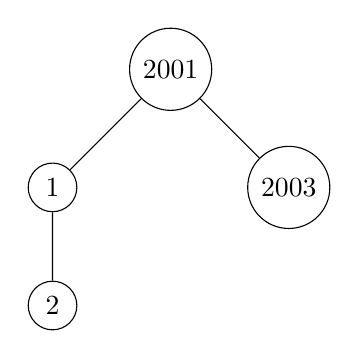
\begin{tikzpicture}[
            level/.style={sibling distance=3cm, level distance=1.5cm},
            every node/.style={draw, circle}
        ]
            \node {2001}
                child { node {1}
                    child { node {2} }
                }
                child { node {2003} };
        \end{tikzpicture}
        \caption{Example AVL Tree}
        \label{fig:enter-label}
    \end{figure}

    
\section{Error Detection}
    \subsection{Invalid input}
        In the parser, if the input is not of the required format, or if the cell row/column is out of bounds we get an invalid input error and status is changed to \texttt{Invalid cmd}

    \subsection{Circular Error}
        As already discussed, the circular error is detected using the AVL Tree, and the status is changed to \texttt{circular error}

    \subsection{Zero Division Error}
        In case we get a zero divison error, we change the isError field of cell struct to true and accordingly print ERR while printing the sheet.

    \subsection{Cells dependent on cells with Zero Division error}
        We detect this while computing the value, just like above we change the isError field to true.
    
    









\end{document}
